%%%%%%%%%%%%%%%%%%%%%%%%%%%%%%%%%%%%%%%%%
% Academic Title Page
% LaTeX Template
% Version 2.0 (17/7/17)
%
% This template was downloaded from:
% http://www.LaTeXTemplates.com
%
% Original author:
% WikiBooks (LaTeX - Title Creation) with modifications by:
% Vel (vel@latextemplates.com)
%
% License:
% CC BY-NC-SA 3.0 (http://creativecommons.org/licenses/by-nc-sa/3.0/)
% 
% Instructions for using this template:
% This title page is capable of being compiled as is. This is not useful for 
% including it in another document. To do this, you have two options: 
%
% 1) Copy/paste everything between \begin{document} and \end{document} 
% starting at \begin{titlepage} and paste this into another LaTeX file where you 
% want your title page.
% OR
% 2) Remove everything outside the \begin{titlepage} and \end{titlepage}, rename
% this file and move it to the same directory as the LaTeX file you wish to add it to. 
% Then add \input{./<new filename>.tex} to your LaTeX file where you want your
% title page.
%
%%%%%%%%%%%%%%%%%%%%%%%%%%%%%%%%%%%%%%%%%

%----------------------------------------------------------------------------------------
%	PACKAGES AND OTHER DOCUMENT CONFIGURATIONS
%----------------------------------------------------------------------------------------

\documentclass[11pt]{report}

\usepackage{lmodern}
\usepackage[utf8]{inputenc} % Required for inputting international characters
\usepackage[T1]{fontenc} % Output font encoding for international characters
\usepackage{blindtext}
\usepackage{tocvsec2}
\usepackage{mathpazo} % Palatino font
\usepackage{hyperref}
\usepackage[parfill]{parskip}
\usepackage{adjustbox}
\usepackage{geometry}
\usepackage{float}
\usepackage{graphicx}

\setcounter{secnumdepth}{3}
\setcounter{tocdepth}{3}

\hypersetup{
    colorlinks=true,
    linkcolor=blue,
    filecolor=magenta,      
    urlcolor=cyan,
    pdftitle={Overleaf Example},
    pdfpagemode=FullScreen,
}

%%%%%%%%%%%%%%%%%%%%% COMMANDS %%%%%%%%%%%%%%%%%%%%%

\newcommand\shortlorem{Lorem ipsum dolor sit amet, consectetur adipiscing elit, sed do eiusmod tempor incididunt ut labore et dolore magna aliqua. Ut enim ad minim veniam, quis nostrud exercitation ullamco laboris nisi ut aliquip ex ea commodo consequat.}

\newcommand{\addchapter}[1]{
	\addcontentsline{toc}{section}{#1}
	\chapter*{#1}
}

\newcommand{\addsection}[1]{
	\addcontentsline{toc}{subsection}{#1}
	\section*{#1}
}

\newcommand{\addsubsection}[1]{
	\addcontentsline{toc}{subsubsection}{#1}
	\subsection*{#1}
}

%%%%%%%%%%%%%%%%%%%%% END COMMANDS %%%%%%%%%%%%%%%%%%%%%

\begin{document}

%----------------------------------------------------------------------------------------
%	TITLE PAGE
%----------------------------------------------------------------------------------------

\begin{titlepage} % Suppresses displaying the page number on the title page and the subsequent page counts as page 1
	\newcommand{\HRule}{\rule{\linewidth}{0.5mm}} % Defines a new command for horizontal lines, change thickness here
	
	\center % Centre everything on the page
	
	%------------------------------------------------
	%	Headings
	%------------------------------------------------
	
	\textsc{\LARGE URV Universitat Rovira i Virgili}\\[0.5cm] % Main heading such as the name of your university/college
	\textsc{\LARGE UOC Universitat oberta de Catalunya}\\[1.5cm]
	
	\textsc{\Large Master in Computational and Mathematical Engineering}\\[0.5cm] % Major heading such as course name
	
	\textsc{\large Final Master Project}\\[0.5cm] % Minor heading such as course title
	
	%------------------------------------------------
	%	Title
	%------------------------------------------------
	
	\HRule\\[0.4cm]
	
	{\huge\bfseries Soundless: A study on noise sleep disturbance}\\[0.4cm] % Title of your document
	
	\HRule\\[1.5cm]
	
	%------------------------------------------------
	%	Author(s)
	%------------------------------------------------
	
	\begin{minipage}{0.4\textwidth}
		\begin{flushleft}
			\large
			\textit{Author}\\
			Santi \textsc{Mart\'inez P\'erez} % Your name
		\end{flushleft}
	\end{minipage}
	~
	\begin{minipage}{0.4\textwidth}
		\begin{flushright}
			\large
			\textit{Supervisor}\\
			Prof. Pedro \textsc{Garc\'ia L\'opez} % Supervisor's name
		\end{flushright}
	\end{minipage}
	
	% If you don't want a supervisor, uncomment the two lines below and comment the code above
	%{\large\textit{Author}}\\
	%John \textsc{Smith} % Your name
	
	%------------------------------------------------
	%	Date
	%------------------------------------------------
	
	\vfill\vfill\vfill % Position the date 3/4 down the remaining page
	
	{\large\today} % Date, change the \today to a set date if you want to be precise
	
	%------------------------------------------------
	%	Logo
	%------------------------------------------------
	
	%\vfill\vfill
	%\includegraphics[width=0.2\textwidth]{placeholder.jpg}\\[1cm] % Include a department/university logo - this will require the graphicx package
	 
	%----------------------------------------------------------------------------------------
	
	\vfill % Push the date up 1/4 of the remaining page
	
\end{titlepage}

%----------------------------------------------------------------------------------------


\tableofcontents

\addchapter{Introduction}
Sleep quality is an important factor for good health. Nowadays the human population is living in megalopolis, with high density population in small areas, giving rise to noisy ambients the 24 hours of the day. Studying how noise can affect sleep quality seems like a worthwhile topic to which we should devote time. The following pages presents a first approach to an sleep quality study.

\addsection{Soundless}
The \href{https://soundless.app}{Soundless} app is a project leaded by Universitat Rovira i Virgili at Tarragona, Spain. The project aims to study how noise affects the sleep quality by providing a bracalet equiped with sensory to monitor vital signs of the subject. Along with the bracalet, an android app is provided to record the sound in the ambient while the bracelet is working. Ideally we must be able to see some arousals in the vital signs signals when high noise is recorded by the mobile application, so we can conclude how noise affects or not the sleep quality. The challenge is, however, not trivial. Since the bracelet will only record oxigen saturation and heart rate, to arrive at any conclusion is hard to do. In top of that the sleep itself is a field of study and a complex topic: there are several stages at sleep, noise may affect differently in different stages. There may be subjects more used to noise in the ambient while sleeping and noise at different frequency ranges may affect differently to different subjects.

Additionally, there are not many subjects in the sounless app study yet, around 20 people participed in the study so we looked for alternatives datasets to start our study.

\addsection{The Human Sleep Project}
\href{https://bdsp.io/content/hsp/2.0/}{The Human Sleep Project} is a project carried out by Massachusetts General Hospital, they are recording several electroencephalograms of subjects with some sleep pathology. The documents, stored in .edf (European Data Format) format are usually accompanied with annotations on the electroencephalograms as well as the channels used for the recording. This is a vast dataset with around 25000 encephalograms to study. With this information makes sense to try to develop some kind of artificial intelligence solution to annotate encephalograms automatically, this is the main focus of this study. At some point, the tecnology used here may help to detect arousals related to noise in the ambient using similar methodologies. 


\addchapter{State of art}
The relationship between environmental noise and sleep quality has been the focus of extensive interdisciplinary research due to its profound implications for public health. Numerous studies have demonstrated that nocturnal noise exposure adversely affects both the physiological and psychological dimensions of sleep, including sleep architecture, duration, and subjective sleep quality.

One of the most influential sources on this topic is the World Health Organization's environmental noise guidelines, which synthesize extensive epidemiological and experimental evidence. Basner and McGuire (2018), in their systematic review, concluded that nighttime exposure to noise from traffic, aircraft, and industrial sources leads to delayed sleep onset, increased number and duration of awakenings, and reduced deep sleep (slow-wave sleep). These findings support earlier work by Muzet (2007), who outlined the biological pathways through which noise interferes with sleep, such as through increased heart rate, blood pressure, and cortical arousals.

Different types of environmental noise have been shown to affect sleep in varying degrees. Griefahn et al. (2006) and Pirrera, De Valck, and Cluydts (2010) reviewed the impacts of road, rail, and air traffic noise, noting that aircraft noise tends to be the most disruptive due to its variability and unpredictability. Basner et al. (2008) used polysomnography to demonstrate that aircraft noise exposure reduces the proportion of REM and slow-wave sleep, both critical for physical recovery and cognitive function.

Recent studies have also investigated the role of individual differences in noise sensitivity. Elmenhorst et al. (2012) found that individuals with higher subjective sensitivity to noise are more prone to awakenings and have lower sleep efficiency under noisy conditions. Similarly, Riedel et al. (2022) showed that noise annoyance significantly moderates the relationship between traffic noise exposure and sleep quality, indicating that psychological factors mediate the perception and physiological impact of noise.

Urbanization and socioeconomic status are additional contextual factors that modulate the effects of noise. Dzhambov et al. (2017), through meta-analysis, found that people living in urban and low-income neighborhoods are disproportionately affected by road traffic noise, suggesting environmental justice implications. Brown and van Kamp (2009) emphasized the role of subjective appraisal and context in shaping noise response, indicating that perceptions of control and expectations may alter physiological responses to the same noise level.

The long-term consequences of chronic noise-induced sleep disruption are also well-documented. Witte et al. (2021) linked prolonged night-time noise exposure to cognitive decline in older adults, while Dratva et al. (2012) showed that noise-related sleep disturbance is associated with reduced health-related quality of life and increased psychological distress.

In sum, the current body of research provides robust evidence that environmental noise impairs sleep quality through both direct physiological mechanisms and mediated psychological pathways. While regulation and mitigation strategies have been proposed, further research is needed to explore personalized interventions and to better understand vulnerable populations.

\addchapter{Implementation}
In this section we will present the different approaches to the problem that have been used in the development process, some of them have been dropped for the poor results obtained, and the last one presented here is the main proposal of the document, giving fair results, and aiming to be a useful tool in electroencephalography classification. Due to the nature of the dataset, more that 25000 files, weighting around 500MB in average, the training process of neural networks presented here is not simple, we need in a first phase to download the data, in a second stage, the data must be treated and aggregated, and finally the network shoud be trained.

The whole \href{https://github.com/szz-dvl/soundless/tree/main}{implementation} is coded in python, a friendly language for IA related tasks, having great libraries such as keras, tensorflow and scikit learn, that we will use extensively.

For the download process, \href{https://pypi.org/project/boto3/}{boto3} library is used to interactuate with AWS s3 instances hosting the data.

To treat the data, \href{https://mne.tools/stable/index.html}{MNE} library is used, this one comes in handy to deal with .edf files, allowing us to get the epochs of an encephalogram related to a particular annotation and computing the PSDs associated with each event.

To aggregate the data a \href{https://www.postgresql.org/}{postgreSQL} DDBB have been used, when the data is downloaded and treated is aggregated in different batches and saved into a relational database, the neural network will read those chunks of data for the training process.

Finally to create the neural networks proposed here \href{https://keras.io/}{keras} is used. This is a great library abstracting the tough part of neural networks and allowing for quick prototipe a neural network. 

\addsection{Feature engineering}
The vast amount of data comming from encephalogram files must be treated before we can feed this data to a neural network.
First of all we need to get a glimpse at the channels used for the encephalogram recording, with some examples we realize that there are several kinds of configurations for encephalograms, a neural network won't work if we do not standardize the data between the different encephalograms. Once we select a set of channels representing the majority of our data set, we need to obtain the different epochs of the encephalograms associated to the annotations. 

\addsubsection{Channel selection}
To select the representative channels of our dataset, we first traverse all our documents looking for the different channels configurations, this process will generate a CSV file with a fingerprint of the channels for each encephalogram, here a fingerprint means nothing but to concatenate all the channel names separated by a "|" character for each encephalogram. This \href{https://github.com/szz-dvl/soundless/blob/main/parser_channels.py}{file} is the responsible for this data gathering process.

Once we have generated the CSV file with one fingerprint per row, we can start analysing the different channel configurations to get a set of desired channels to study. The process is coded in this \href{https://github.com/szz-dvl/soundless/blob/main/channels.py}{file}. Roughly, this file will make an study of the frequency of each channel present in the dataset, and will try to llok for equivalent channels, two channels are considered equivalent when two different configurations are equal by exchanging this channels. The results obtained in this process are as follows:

\begin{table}[!h]
\begin{center}
\begin{tabular}{ |p{3cm}||p{3cm}| }
 \hline
 Channel & Frequency (\%)\\
 \hline
 ABD & 88.719512 \\ 
 AIRFLOW & 75.304878 \\  
 C3-M2 & 71.951220 \\
 CHEST & 87.042683 \\
 E1-M2 & 84.451220 \\
 EKG & 87.957317 \\
 HR & 89.786585 \\
 IC & 89.329268 \\
 LAT & 82.164634 \\
 O1-M2 & 70.731707 \\
 RAT & 79.878049 \\
 SNORE & 91.920732 \\
 SaO2 & 90.396341 \\
 \hline
\end{tabular}
\end{center}
\caption{Channel frequencies}
\label{tab1}
\end{table}

So, demanding that our encephalograms have, at least, this channels we must get a representation of around a 71\% of our dataset, which must be more than enough to train our neural network. Following with the obtained results, the meaningful equivalences found are as follows:

\newgeometry{left=1.5cm,bottom=1.5cm,top=0.5cm}
\begin{minipage}{0.45\textwidth}
\begin{adjustbox}{angle=90}
\begin{tabular}{ |p{2cm}||p{3cm}||p{2cm}||p{2cm}||p{2cm}||p{2cm}||p{2cm}||p{2cm}||p{2cm}| }
 \hline
 \multicolumn{9}{|c|}{Channel equivalences} \\
 \hline
 C4-M1 \newline C4-M2 & CHIN1-CHIN2 \newline CHIN1-CHIN3 \newline CHIN2-CHIN3 \newline CHIN3-CHIN1 \newline CHIN3-CHIN2 \newline Chin1-31 \newline Chin1-Chin2 \newline Chin1-Chin3 \newline Chin1-P3 \newline Chin1-P4 \newline Chin2-Chin3 \newline Chin3-Chin2 & E1-M1 \newline E1-M2 & E2-M1 \newline E2-M2 & EKG \newline EKG-E1 & F4-M1 \newline F4-M2 \newline F8-M1 \newline Fp2-M1 \newline Fp2-M2 & O2-M2 \newline O1-M1 \newline O2-M1 & LAT \newline LAT-E1 & RAT \newline RAT-E1 \\ 
 \hline
\end{tabular}
\end{adjustbox}
\end{minipage}%
\hfill
\begin{minipage}{0.45\textwidth}
\begin{table}[H]
\begin{center}
\begin{tabular}{ |p{3cm}||p{3cm}||p{3cm}| }
 \hline
 Channel & Frequency (\%) & Equivalence\\
 \hline
 ABD & 88.719512 & No \\ 
 AIRFLOW & 75.304878 & No \\  
 C3-M2 & 71.951220 & No \\
 C4-M1 & 76.371951 & Yes \\
 CHEST & 87.042683 & No \\
 CHIN1-CHIN2 & 91.310976 & Yes \\
 E1-M1 & 85.365854 & Yes \\
 E2-M1 & 87.347561 & Yes \\
 EKG & 90.396341 & Yes \\
 F4-M1 & 81.402439 & Yes \\
 HR & 89.786585 & No \\
 IC & 89.329268 & No \\
 LAT & 84.451220 & Yes \\
 O1-M2 & 70.731707 & No \\
 O2-M2 & 86.280488 & Yes \\
 RAT & 82.164634 & Yes \\
 SNORE & 91.920732 & No \\
 SaO2 & 90.396341 & No \\
 \hline
\end{tabular}
\end{center}
\caption{Frequencies with equivalences aggregated}
\label{tab2}
\end{table}
\end{minipage}%
\restoregeometry

In table \autoref{tab2} I sumarize the frequencies obtained when aggregating the equivalences found by the code, after all we have 18 meaningful channels to play with, however we need to take into account that most of them are not electroencephalogram channels, so looking for brain activity on those channels will make no sense, we will review this part later on. However we can try to use the 18 channels to feed a neural network as they are, as a sequence of voltages per channel over time. 

\addsubsection{Classes}
If we take a look at the annotation documents associated to each encephalogram there is a huge number of distinct annotations for the whole set, however if we look carefully, we realise that the most prevalent annotations in all the encephalograms are the sleeping stages. It makes sense to try to classify the sleeping stages of a subject, the sleeping stages are:

\begin{itemize}
  \item \textbf{Sleep\_stage\_W:} This stage indicates that the subject is awake.
  \item \textbf{Sleep\_stage\_N1:} This stage indicates that the subject is in the first sleep stage.
  \item \textbf{Sleep\_stage\_N2:} This stage indicates that the subject is in the second sleep stage.
  \item \textbf{Sleep\_stage\_N3:} This stage indicates that the subject is in the third sleep stage.
  \item \textbf{Sleep\_stage\_R:} This stage indicates that the subject is in REM (Rapid Eye Movement) stage.
\end{itemize} 

So these will be our class set, lets try to classify our encephalogram events into one of these stages. We can try to use a similar method to look for diferent kind of arousals in the encephalograms and, later on, try to associate those arousals to noise in the ambient.

\addsection{Fully Convolutional neural network (FCN)}
Based on \href{https://arxiv.org/abs/1611.06455}{this} paper and the related work found \href{https://keras.io/examples/timeseries/eeg_signal_classification/}{here} I tried to build a fully convolutional network for timeseries classification, the architecture is as follows:

\begin{figure}[H]
\centering
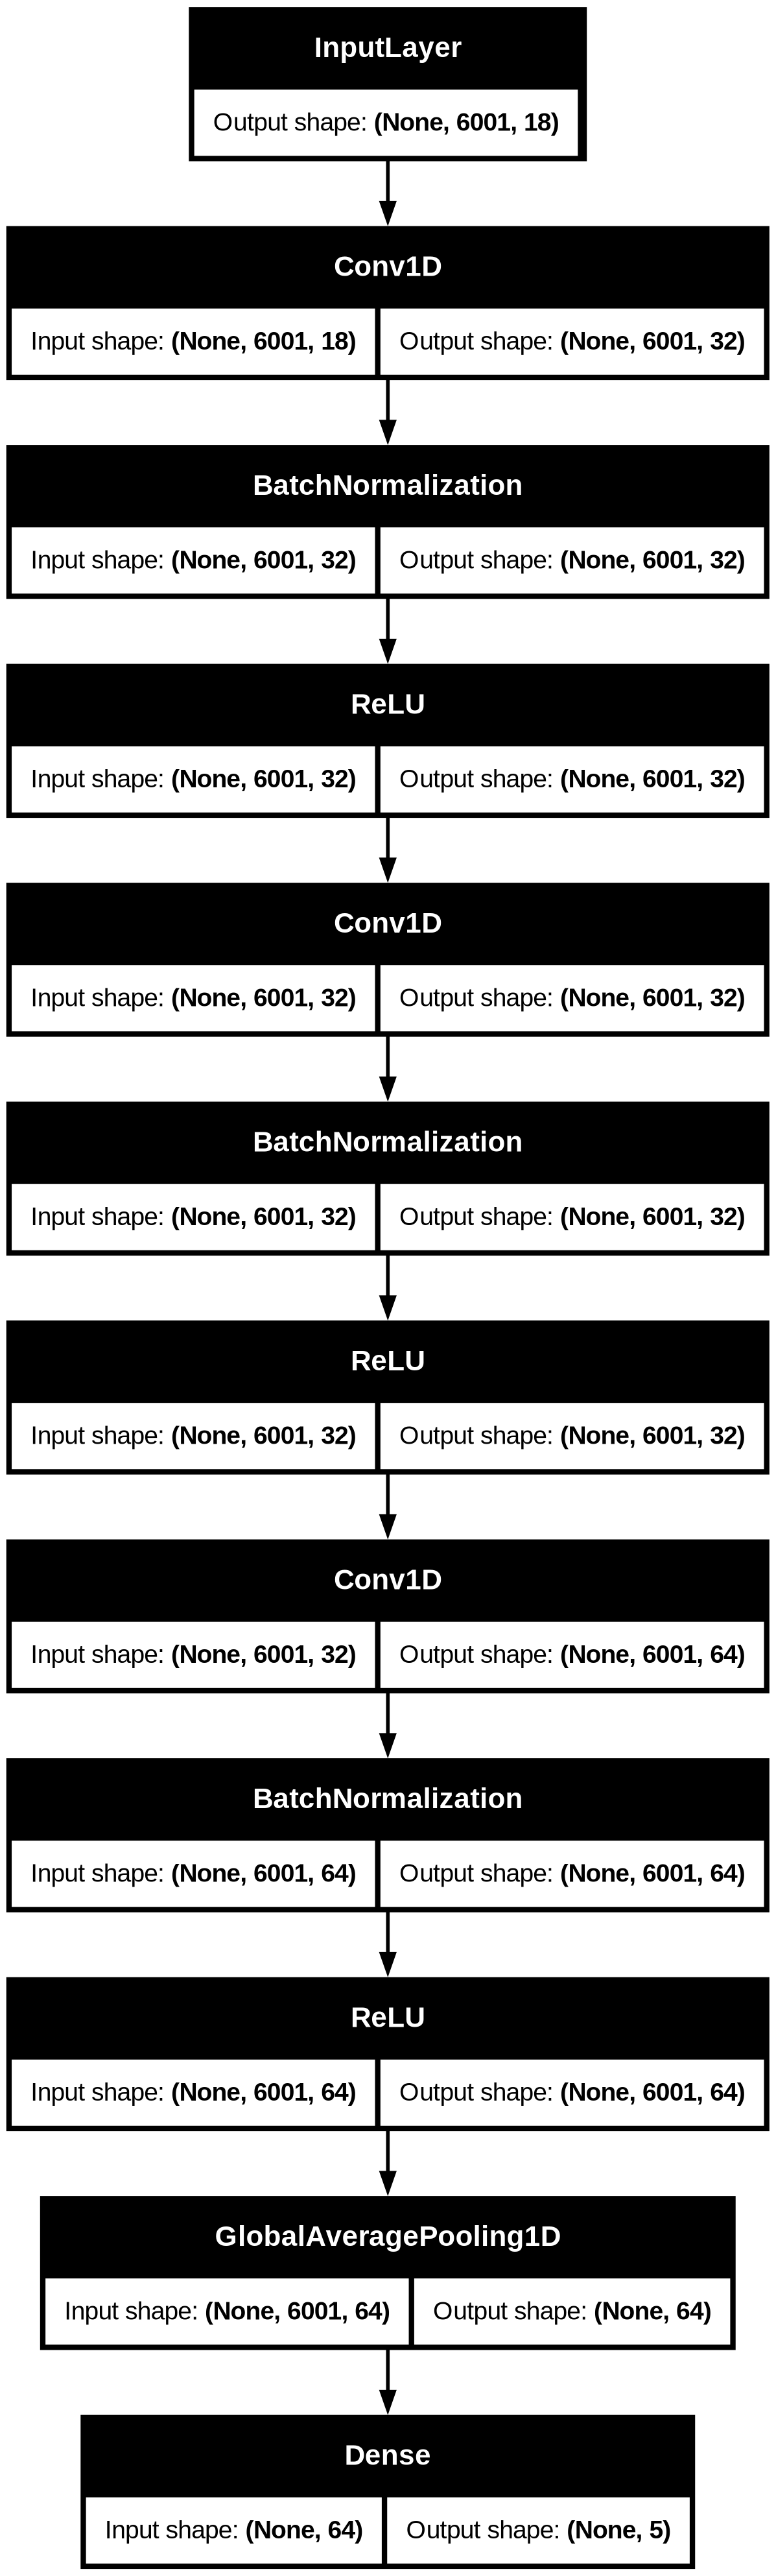
\includegraphics[scale=.1, angle=90]{figs/fcn.png}
\caption{FCN architecture}
\label{fig1}
\end{figure}

The input shape is (6001, 18) given that we have 18 channels and that we are annalising cropped segments of the encephalogram 30 seconds long. The sample frequency of the encephalograms is 200 Hz, so we have 6000 samples per event. Any encephalogram found with a different sample frequency will be discarted in this approach. Then we have a convolutional layer of 32 filters with a kernel size of 3. After that another convolutional layer with again 32 filters and a kernel size of 5. Finally we use a last convolutional layer with 64 filters and a kernel size of 5. Then we use an average pooling layer to downsample the results of convulational layers. Finally a dense layer with 5 neurons, the number of classes we would like to classificate.

The activation function I'm using for the hidden layers of the network is \href{https://en.wikipedia.org/wiki/Rectifier_(neural_networks)}{ReLU}(rectified linear unit) since is very efficient and mitigates the \href{https://en.wikipedia.org/wiki/Vanishing_gradient_problem}{vanishing gradient} problem. For the output layer softmax is used, since we have a multiclass classification problem.

The parameters of this neural network have been optimized by using \href{https://keras.io/keras_tuner/}{keras tuner} a tool to automate the process of selecting the hyperparameters of our network. It is not perfect for us since we are dealing with a huge dataset hosted elsewhere, so we need to tune the model with a few samples of the dataset, but is a helping tool anyway.

Several options have been tried for the optimizer with this architecture. In particular Adam, SGD (Stochastic gradient descen) and AdamW with a weight decay of 1e-4. At the same time several learning rate values ranging from 1e-3 to 1e-5 have been tried and a \href{https://keras.io/api/callbacks/learning_rate_scheduler/}{LearningRateScheduler} have been applied too.

After one day of training this approach could not overcome a 20\% of validation accuracy, which is not better than a random choice of one of our classes. We need to take into account that we are feeding the network with a very different selection of channels what will probably lead to a very noisy data set. After applying data scalation with MinMax scaler the accuracy improved a bit, but still not enough to make it a useful tool.

\addsubsection{LSTM}
\href{https://en.wikipedia.org/wiki/Long_short-term_memory}{LSTM} (Long short-term memory) neural networks are a kind of recurrent neural network that are very well suited for time series classification, by using an LSTM layer instead of our 2 last convolutional layers we may get better results. The architecture proposed is as follows:

\begin{figure}[H]
\centering
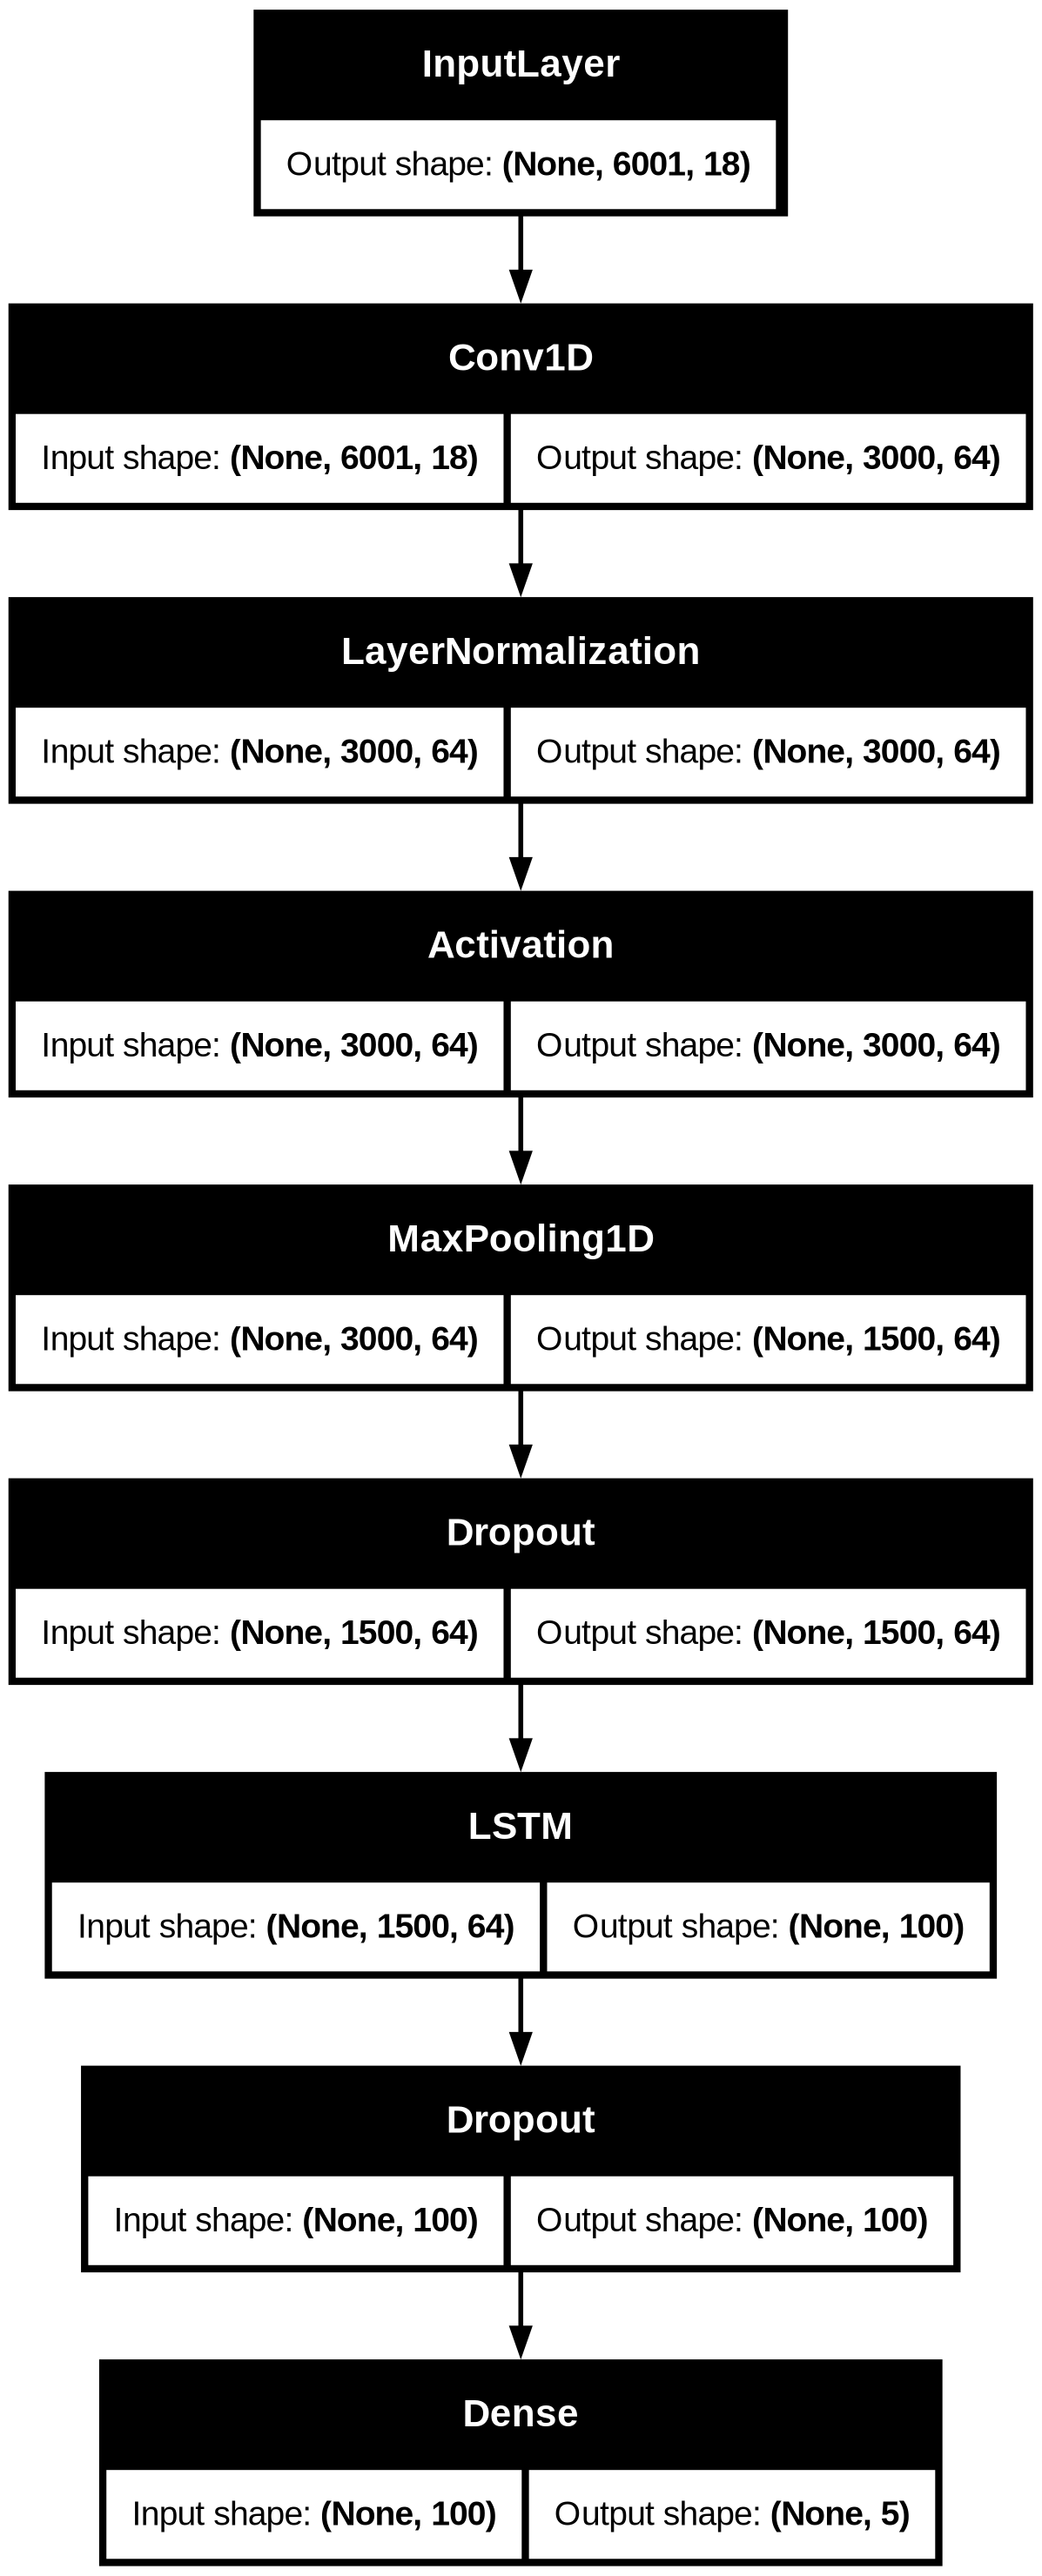
\includegraphics[scale=.1, angle=90]{figs/fcn-lstm.png}
\caption{CN-LSTM architecture}
\label{fig2}
\end{figure}

We keep the same input layer, with shape (6001, 18). After that we use an initial convolutional layer with 64 filters and a kernel size of 3, which is good at learning general patterns in our data after that we use a normalization layer that we connect with a ReLU activation layer, finally we use a pooling layer to downsample the results obtained in this first step. After that we connect a droput layer to avoid overfiting, this layer will "deactivate" a percentage of the neurons of the interconnected layers to trying to avoid that the weights of our gradient are too much affected by noisy data. After that we plug the LSTM layer with 100 neurons and the default tanh activation function, a dropout layer is added after this one and finally we have the output layer, with 5 neurons, again the number of classes we would like to classify.

For this architecture several optimizers has been tried too, particullarly Adam with learning rates ranging from 1e-3 to 1e-5 and AdamW with a weight decay of 1e-4.

After several days training this architecture was not able to overcome 45\% in validation accuracy, an improvement over fully convolutional neural networks, not enough however.

\addsection{Band power aggregation}
Until now I did not have too much success, a 45\% on validation accuracy is still not a good result. Most probably we are dealing with very noisy data not representative of the sleep stage in the subjects, as an instance ABD or IC channels does not seem a good choice to study the sleep stages of a subject. In top of that try to feed a neural network with the raw readings of an encephalogram seems a pretty poor choice, since there may be a lot of artifacts messing our data.

We can think in an encephalogram as a bunch of signals, but, the brain activity is characterized by particular frequencies appearing or desapearing at different moments in the brain, if we were able to study the influence of those frequencies en each of our events we will have a much more cleaner dataset.

\addsubsection{Delta activity}
Delta brainwaves, also known as delta activity, are the slowest brainwaves, typically between 0.5 and 4.5 Hz. They are primarily associated with deep, dreamless sleep, where the body is in a state of complete relaxation and the mind is minimally active. Delta waves are also observed in newborns, and can be induced in a waking state by experienced meditators.

They usually show a high amplitude and are most prevalent during deep sleep stages (3), where the brain is essentially shut down for repair and regeneration. Delta waves are linked to various restorative processes, including tissue repair, muscle growth, and hormone release.They are also involved in transferring information from the hippocampus to the neocortex, aiding in long-term memory storage.

\addsubsection{Theta activity}
Theta brainwaves, characterized by frequencies between 4.5-8.5 Hz, are associated with states of relaxation, deep meditation, and creativity. They are often observed during sleep, particularly during dream sleep, and are also linked to states of daydreaming and focused attention. Theta activity is thought to play a role in processing information, making memories, and facilitating intuitive insights. 

Disrupted or divergent theta activity has been linked to various mental health conditions.

\addsubsection{Alpha activity}
Alpha brainwaves, with a frequency of 8.5-11.5 Hz, are associated with a relaxed, awake state, often observed during activities like daydreaming or meditation. They indicate the brain is active but not overly focused, promoting feelings of calmness and ease. 

Alpha activity is typically strongest over the posterior areas of the head, particularly the occipital cortex. Alpha waves can be influenced by various factors, including sensory stimuli, mental activities, and even the position of the eyes (they are often more prominent with eyes closed). 

\addsubsection{Sigma activity}
Sigma activity, also known as sigma power or spindle activity, refers to brainwave activity in the frequency range of 11.5-15.5 Hz, a key component of non-REM sleep. These brainwaves are characterized by transient oscillations and are often associated with sleep-dependent memory consolidation and sleep stability. In infants, sigma activity is linked to psychomotor development and local brain maturation.

\addsubsection{Beta activity}
Beta activity in the brain refers to a range of brainwave frequencies, typically between 15.5 and 30 Hz, associated with alert, focused, and active mental states. These brainwaves are commonly present during waking hours and when engaged in tasks requiring concentration, problem-solving, or decision-making.

An excessive beta activity can be associated with symptoms of brain over-arousal, such as anxiety, obsessiveness, and sleep difficulties, while a deficient beta activity may be linked to difficulties concentrating, problem-solving, and overall brain under-arousal.

\addsection{Power Spectral Density (PSD)}
Power Spectral Density (PSD) analysis is used to examine the spectral composition of EEG signals during sleep, providing insights into different sleep stages and potential sleep disorders. It's a quantitative EEG (qEEG) technique that measures the distribution of power across different frequency bands within the EEG signal.

Inspired by \href{https://mne.tools/stable/auto_tutorials/clinical/60_sleep.html#design-a-scikit-learn-transformer-from-a-python-function}{this} article, I used the frequencies spectrum derivated from the PSD analisys of the EEGs, obtaining a vector of "features" characterizing which amount of power we find in each channel for the frequencies related to brain activity.

However, the channels we were using until the moment are not the best choice to look for brain activity, hence the list of meaningfull channels we will study has been cropped into an smaller but more representative list, the channels we will use for PSD Analisys are the following:

\begin{table}[H]
\begin{center}
\begin{tabular}{ |p{3cm}||p{3cm}||p{3cm}| }
 \hline
 Channel & Frequency (\%) & Equivalence\\
 \hline  
 C3-M2 & 71.951220 & No \\
 C4-M1 & 76.371951 & Yes \\
 E1-M1 & 85.365854 & Yes \\
 E2-M1 & 87.347561 & Yes \\
 F4-M1 & 81.402439 & Yes \\
 O1-M2 & 70.731707 & No \\
 O2-M2 & 86.280488 & Yes \\
 \hline
\end{tabular}
\end{center}
\caption{Channels for PSD Analisys}
\label{tab3}
\end{table}

By computing the PSD of the electroencephalograms for this channels we will obtain a vector of 35 features, the amount of power in each of the brain related activity frequencies (presented above) for each of the channels, we will dircard any other frequency range.

This time we have a much cleaner and representative dataset, we must, however think in a new network architecture that fits better with our new dataset.

\addsection{Multi Layer Perceptron (MLP)}
A Multi Layer Perceptron (\href{https://en.wikipedia.org/wiki/Multilayer_perceptron}{MLP}) is a feed forward neural network, characterized for having an input layer, several hidden layers and an output layer. This kind of neural networs are very well suited for classifing tabulated data. After our PSD analisys we are getting a vector of fixed "features" representing the amount of power of each frequency associated with the brain activity for each of the channels we are studing, a simple MLP must do the job properly, this time the architecture used is the following:

\begin{figure}[H]
\centering
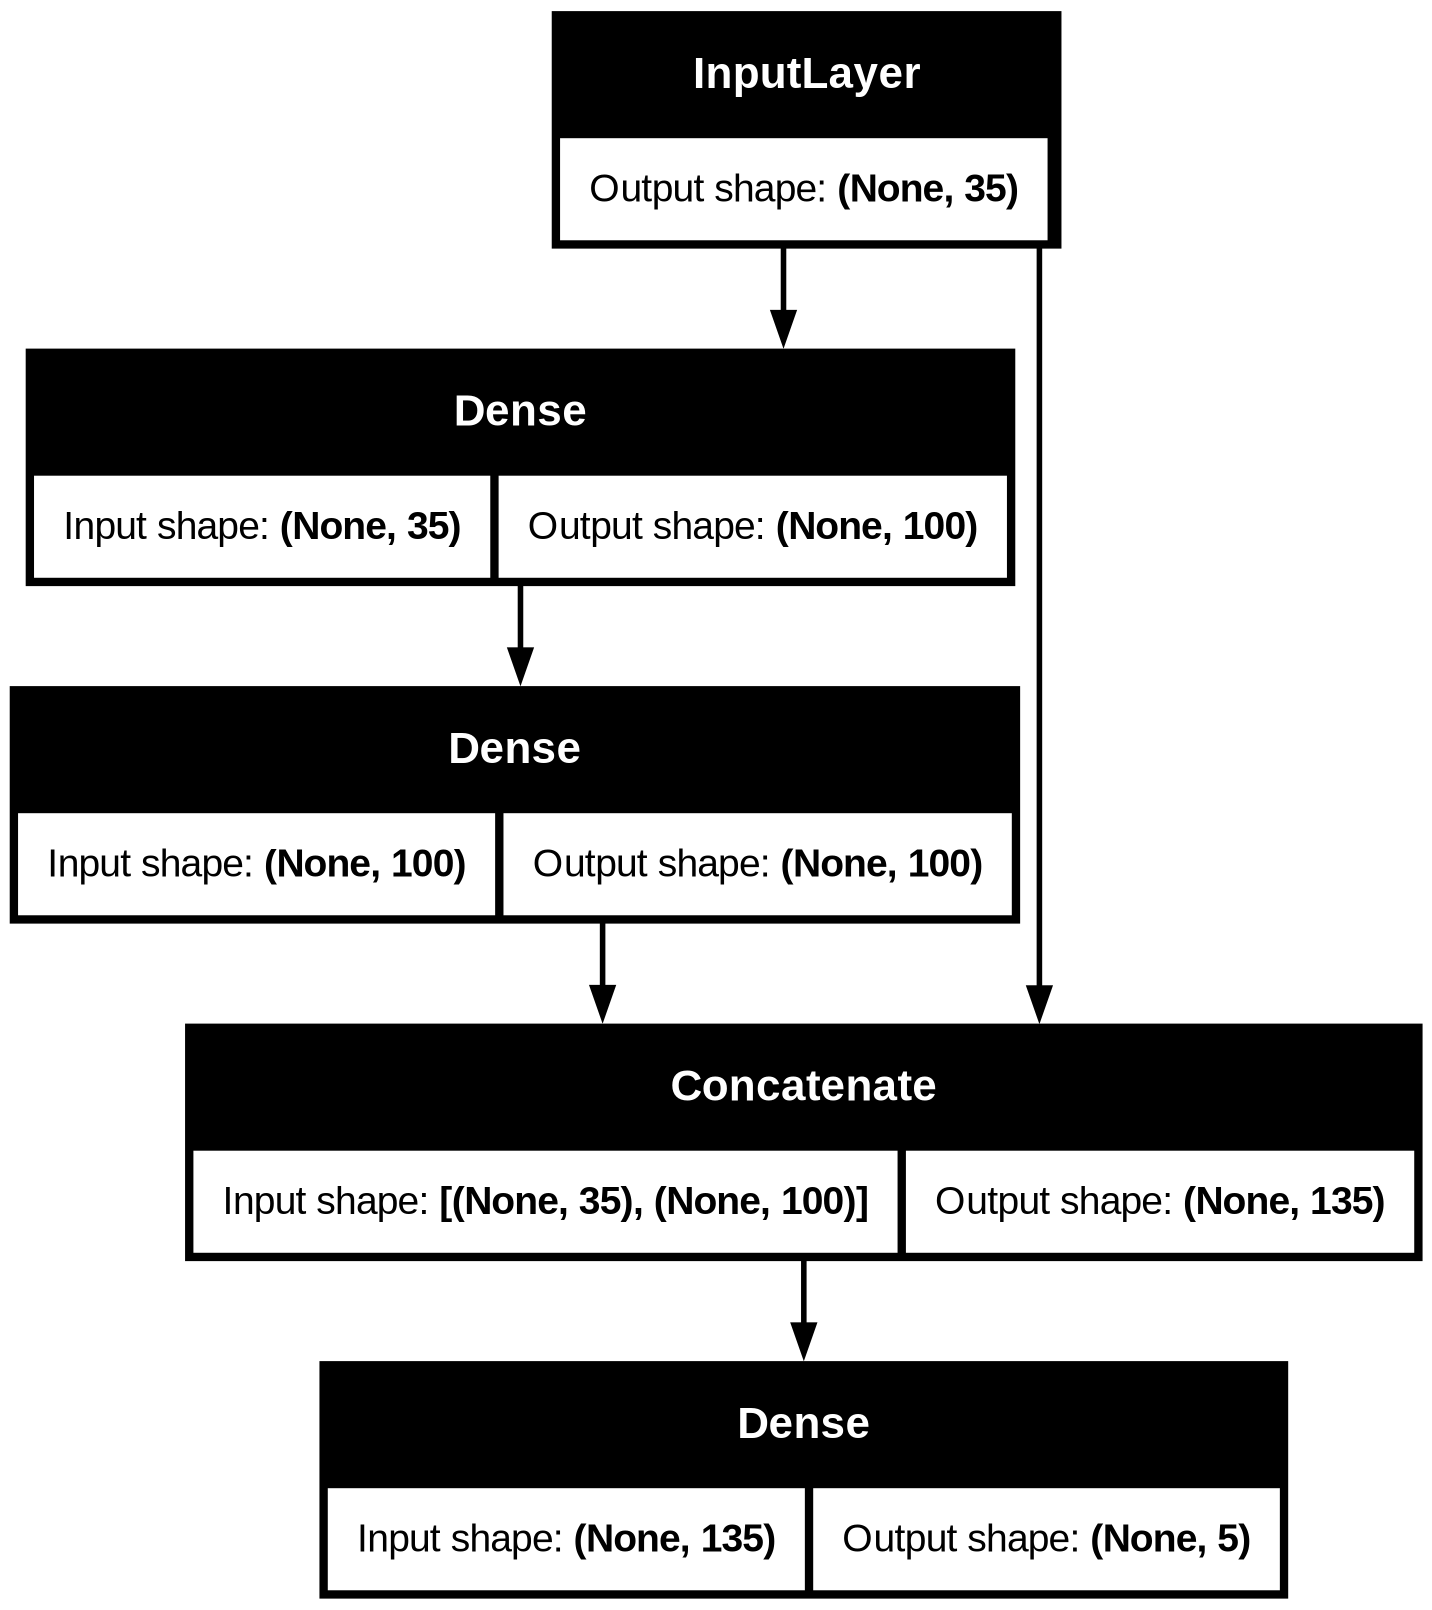
\includegraphics[scale=.2, angle=90]{figs/mlp.png}
\caption{MLP architecture}
\label{fig3}
\end{figure}

We first have our input layer of shape (35), since we have 7 channels multiplied by the 5 frequencies we are interested in. The input is then connected to a first dense layer with 100 neurons and using the ReLU activation function, following another hidden layer of again 100 neurons and using the ReLU activation function. After the dense layers, the input is concatenated with the ouput of the hidden layers, so we have a deep path and a wide path for the data, this use to help the classification process when our input is very representative what we are willing to predict. Finally a dense layer with 5 neurons and an activation function of softmax is attached to the network.

The optimizer used for the MLP is Adam with an initial leraning rate of 1e-3, however a \href{https://keras.io/api/callbacks/reduce_lr_on_plateau/}{ReduceLROnPlateau} is in use to reduce the learning rate when our error is not improving, allowing the network to focus more and to more stable but slow convergence.

The parameters for the number of neurons and the leraning rate for this network have been optimized using \href{https://keras.io/keras_tuner/}{keras tuner}.

\addchapter{Evaluation}
At the moment of writing, the MLP has been trained with 1437 subjects, with, in average, around 850 events each patient what results in more that 1.2M events. we are reaching an accuracy of nearly a 70\% in the validation phase. Now, the tests have been performed in 124 subjects taken randomly from the dataset, with about 102000 events, those subjects are nod feed into the neural network at training stage.

The \href{https://scikit-learn.org/stable/modules/generated/sklearn.metrics.classification_report.html}{classification report} obtained for the predictions computed with the resulting model is the following:

\begin{table}[H]
\begin{center}
\begin{tabular}{ |p{3cm}||p{2cm}||p{2cm}||p{2cm}||p{2cm}| }
 \hline
 & precision & recall & f1-score & support\\
 \hline  
 Sleep\_stage\_W & 0.59 & 0.60 & 0.60 & 13843 \\
 Sleep\_stage\_N1 & 0.33 & 0.26 & 0.29 & 10978 \\
 Sleep\_stage\_N2 & 0.80 & 0.77 & 0.78 & 47168 \\
 Sleep\_stage\_N3 & 0.70 & 0.73 & 0.71 & 13242 \\
 Sleep\_stage\_R & 0.65 & 0.78 & 0.71 & 17240 \\
 & & & & \\
 accuracy &  &  & 0.69 & 102471 \\
 macro avg & 0.61 & 0.63 & 0.62 & 102471 \\
 weighted avg & 0.68 & 0.69 & 0.68 & 102471 \\
 \hline
\end{tabular}
\end{center}
\caption{Classification report}
\label{tab4}
\end{table}

As we can see, our main problem is with class Sleep\_stage\_N1, where we get a precision of 33\%, if we look closely into the classification report we observe that the class is the class with less support, probably applying some data augmentation techniques, like \href{https://imbalanced-learn.org/stable/references/generated/imblearn.over_sampling.SMOTE.html}{SMOTE} will help the neural network to predict better for this class.

The confusion matrix obtained in the trainning is the following:

\begin{figure}[H]
\hspace*{-4cm}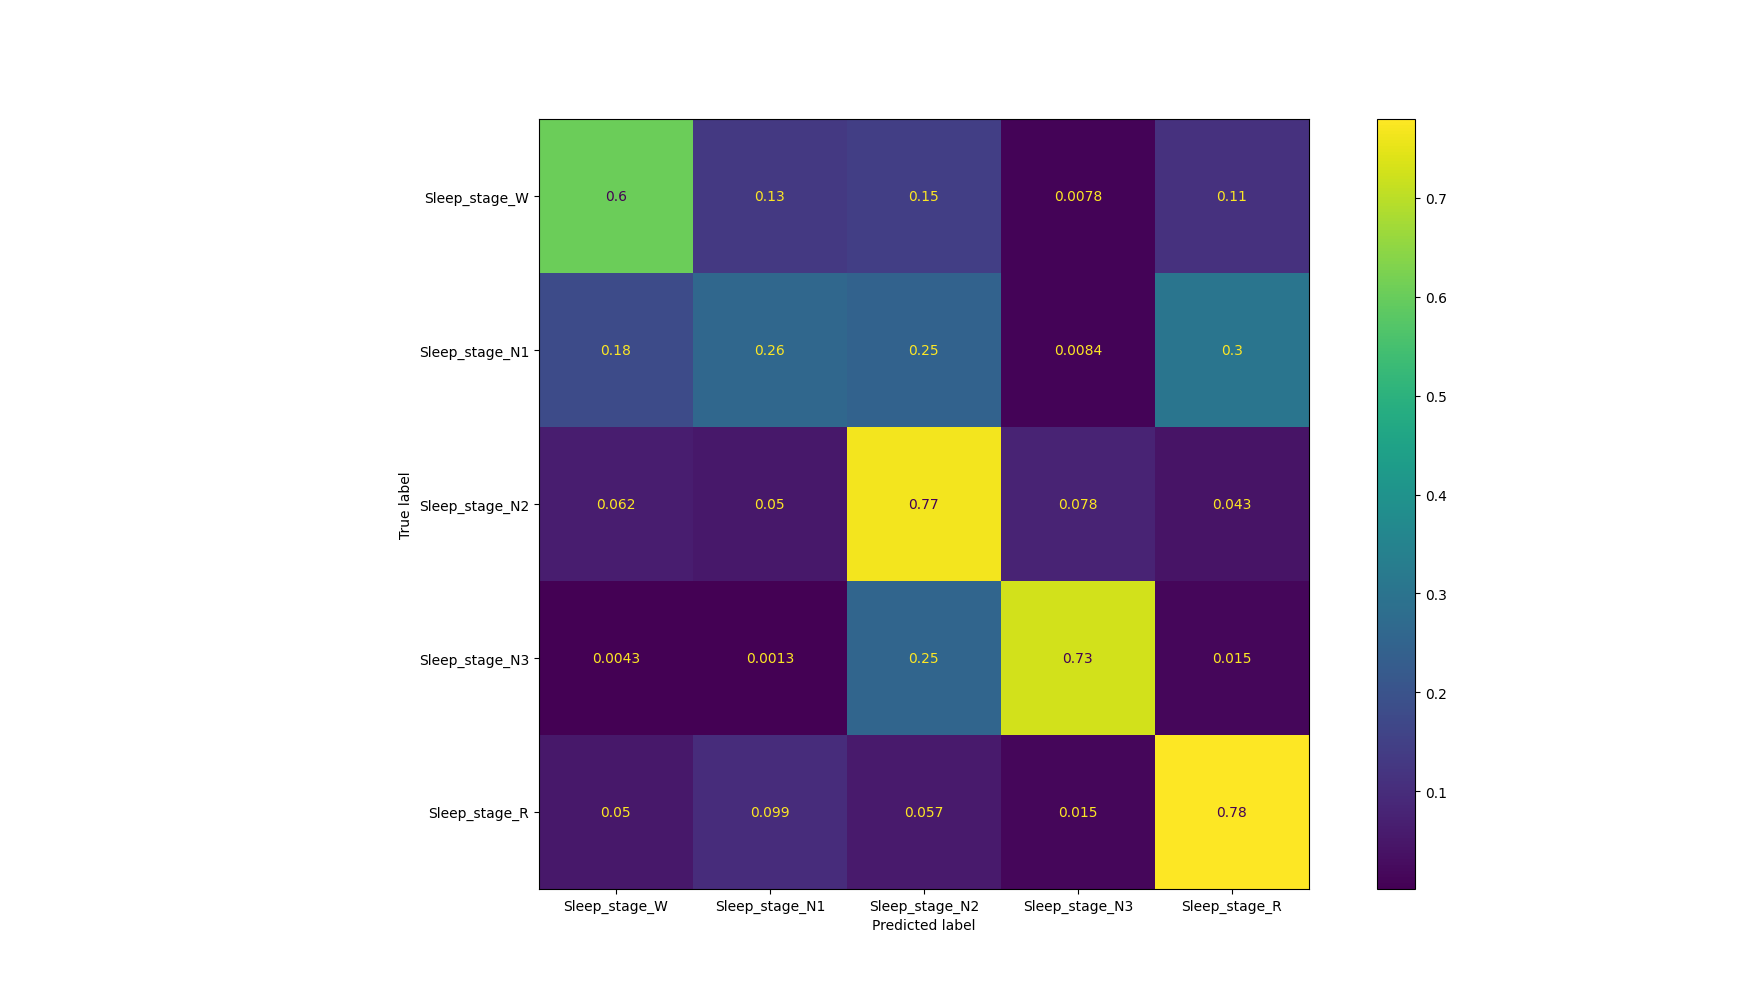
\includegraphics[scale=.5]{figs/cm.png}
\caption{Confussion matrix}
\label{fig4}
\end{figure}

Here we can appreciate that our classifier is not performing well for the Sleep\_stage\_N1 class, being confused mainly with the class Sleep\_stage\_R and Sleep\_stage\_N2. The rest of the classes shows a better perfomance, being Sleep\_stage\_N2, Sleep\_stage\_N3 and Sleep\_stage\_R above the 70\% of success in the prediction.

\addsection{Data augmentation}
Data augmentation or oversampling is a technique that generates synthetic samples for a given dataset, this synthetic samples are generated according to the samples we already have from the target class. To try to mitigate the problem found in the evaluation section with the class Sleep\_stage\_N1 I'm generating synthetic samples exclusively for this class to see if the network performance can be improved for this events.

Estoy trabajando en este apartado

\blindtext

\addchapter{Conclusion}
Sleep study is a complex topic, and how noise affects sleep increases the complexity of such an study. In this document however, we applied a set of techniques that allow us to predict the sleep stage of a subject given an electroencephalogram. 

This techniques can be adapted or extended to study the noise disturbance on a subject while sleeping. As an instance we could categorize and classify the different arousals found in an electroencephalogram and compare the results with a recording with an standard microphone. Actually, the SNORE channel present in most of the electroencephalograms of the The Human Sleep project dataset is a microphone to capture snoring volume during sleep, however we need to take into account that this electroencephalograms has been captured in a very controled environment, so use this recordings to comparate the sounds, probably emitted by the subject itself, with arousals will probably lead to poor results, since the arousals related to snoring may not be related to noise particullarly. Ideally, with similar montages we can achieve what we want, exposing the subjects to sounds at different frequencies and amplitudes we may get a desirable result for this study. World is not ideal, neither is the data, so with the working dataset of the human sleep project this is a first step towards gaining some knowledge on how the noise affect the sleep quality.

\addchapter{Future work}
As concluded above, the techniques used in this study may be a first step towards gaining some knowledge on how the noise affects the sleep quality. By classifing the sleep stages of a subject given an electroencephalogram we can stablish in which period the noise affects more or less a subject. Besides, the gerealization on sleep stage classification, it is, being able to predict the sleep stage of a subject given other subjects data is a great capability, the way we predict sleep stages we can predict arousals given another subject data. Arousal prediction will be another step forward to gain knowledge on how noise affects the sleep quality. 

With a bigger dataset we could use soundless data to make a deeper study on the noise in the ambient, probably by taking the power of sound at different frequencies and trying to detect abnormalities in the signals registered by the bracalet, however, an electroencephalogarm is ideal to study how sleep occurs during the resting hours. 

Further steps from this study may include growing the sounless dataset, detecting arousals from vital signals and trying to stablish a relationship between soundless data and electroencephalogram data. Morover, the dataset from The Human Sleep Project provides, in some cases, a pre-sleep questionary. This questionary could be used to create a user profile, so if soundless users are willing to respond a questionary similar to those provided by The Human Sleep Project it will be a good point to start to relate data between the two datasets.  

\begin{thebibliography}{9}
\bibitem{who}
Basner, M., \& McGuire, S. (2018). WHO environmental noise guidelines for the European region: A systematic review on environmental noise and effects on sleep. International Journal of Environmental Research and Public Health, 15(3), 519.

\bibitem{basner}
Basner, M., Müller, U., \& Elmenhorst, E.-M. (2008). Single and combined effects of air, road, and rail traffic noise on sleep and recuperation. Sleep, 31(4), 513–523.

\bibitem{brown}
Brown, A. L., \& van Kamp, I. (2009). Response to noise in urban environments: How important are context and perception? Journal of Environmental Psychology, 29(1), 1–9.

\bibitem{dratva}
Dratva, J., Zemp, E., Felber Dietrich, D., Bridevaux, P. O., Rochat, T., Schindler, C., \& Gerbase, M. W. (2012). Impact of road traffic noise annoyance on health-related quality of life: Results from a population-based study. Quality of Life Research, 21(6), 1055–1061.

\bibitem{dzhambov}
Dzhambov, A. M., Dimitrova, D. D., \& Dimitrakova, E. D. (2017). Road traffic noise and annoyance: A systematic review and meta-analysis. Noise and Health, 19(87), 105–119.

\bibitem{Elmenhorst}
Elmenhorst, E.-M., Pennig, S., Rolny, V., Quehl, J., Mueller, U., Maass, H., \& Basner, M. (2012). Examining nocturnal railway noise and aircraft noise in the field: Sleep, psychomotor performance, and annoyance. Science of the Total Environment, 424, 48–56.

\bibitem{griefahn}
Griefahn, B., Bröde, P., Marks, A., \& Basner, M. (2006). Autonomic arousals related to traffic noise during sleep. Sleep, 29(4), 531–537.

\bibitem{halperin}
Halperin, D. (2014). Environmental noise and sleep disturbances: A threat to health? Sleep Science, 7(4), 209–212.

\bibitem{muzet}
Muzet, A. (2007). Environmental noise, sleep and health. Sleep Medicine Reviews, 11(2), 135–142.

\bibitem{pirrera}
Pirrera, S., De Valck, E., \& Cluydts, R. (2010). Nocturnal road traffic noise: A review on its assessment and consequences on sleep. Biological Psychology, 84(3), 229–237.

\bibitem{riedel}
Riedel, N., Babisch, W., Gurris, N., \& Greiser, E. (2022). Noise annoyance modifies the association between nocturnal traffic noise and sleep quality. International Journal of Hygiene and Environmental Health, 239, 113902.

\bibitem{witte}
Witte, M., Winkler, A., \& Hage, S. R. (2021). Nocturnal noise exposure and cognitive decline in older adults: A longitudinal population-based study. Environmental Research, 196, 110973.

\bibitem{atlas}
Hrayr P. Attarian \& Nidhi S. Undevia. Atlas of Electroencephalography in Sleep Medicine. 

\bibitem{keras}
Suvaditya M. Electroencephalogram Signal Classification for action identification. Available at: \href{https://keras.io/examples/timeseries/eeg_signal_classification/}{https://keras.io/examples/timeseries/eeg\_signal\_classification/}

\bibitem{mne}
Alexandre Gramfort, Stanislas Chambon \& Joan Massich. Sleep stage classification from polysomnography (PSG) data. Available at: \href{https://mne.tools/stable/auto_tutorials/clinical/60_sleep.html}{https://mne.tools/stable/auto\_tutorials/clinical/60\_sleep.html}

\bibitem{timeseries}
Zhiguang Wang, Weizhong Yan \& Tim Oates. Time Series Classification from Scratch with Deep Neural Networks: A Strong Baseline. Available at: \href{https://arxiv.org/abs/1611.06455}{https://arxiv.org/abs/1611.06455}

\bibitem{mlp}
Jiacheng Hou, Zhenjie Song \& Ercan Engin Kuruoglu. BrainNetMLP: An Efficient and Effective Baseline for Functional Brain Network Classification. Available at: \href{https://arxiv.org/pdf/2505.11538}{https://arxiv.org/pdf/2505.11538}

\end{thebibliography}
\end{document}
